\section{Design}\label{design}



\subsection{Interface}


Developers using \sys{} write function handlers and define triggers
just like they would for any existing serverless offering. In addition, they 

Developers express priorities to \sys{} by assigning functions a price value,
which they are willing to pay per unit time that the job spends running. The
price implicitly tells \sys{} the job's priority, in a way that enables \sys{}
to directly compare the priorities of two functions of different tenants. This
also creates an incentive for developers to not only always choose the highest
priority, they have to be willing to pay for it. In order to avoid an escalating
bidding war among developers, \sys{} exposes only a fixed list of possible
prices that developers choose from. For instance, in the example of the web
server, the home page view might be assigned a higher priority and cost
2$\mu\cent$ per cpu second, a the user profile view might be a assigned a
middle-high priority and cost 1.5$\mu\cent$ per cpu second, and finally the
image processing job can be set to a low priority which costs only 0.5$\mu\cent$
per cpu second. 

\Sys{} ensures that the priority of a request is inherited in order to avoid
priority inversion: if a high priority job calls a usually low priority job
synchronously, \sys{} will run the low priority job with high priority for that
invocation.

Developers are also required to express a maximum amount of memory per function.
 
To avoid unexpected costs in the case of for example a DOS attack or a bug,
developers also express a monthly budget that they are willing to pay.\ \sys{}
uses this budget as a guideline and throttles invocations or decreases quality
of service in the case that usage is not within reason given the expected
budget, though it does not guarantee that the budget will not be exceeded by
small amounts.



\subsection{\Sys{} Design}

\begin{figure}[t]
    \centering
      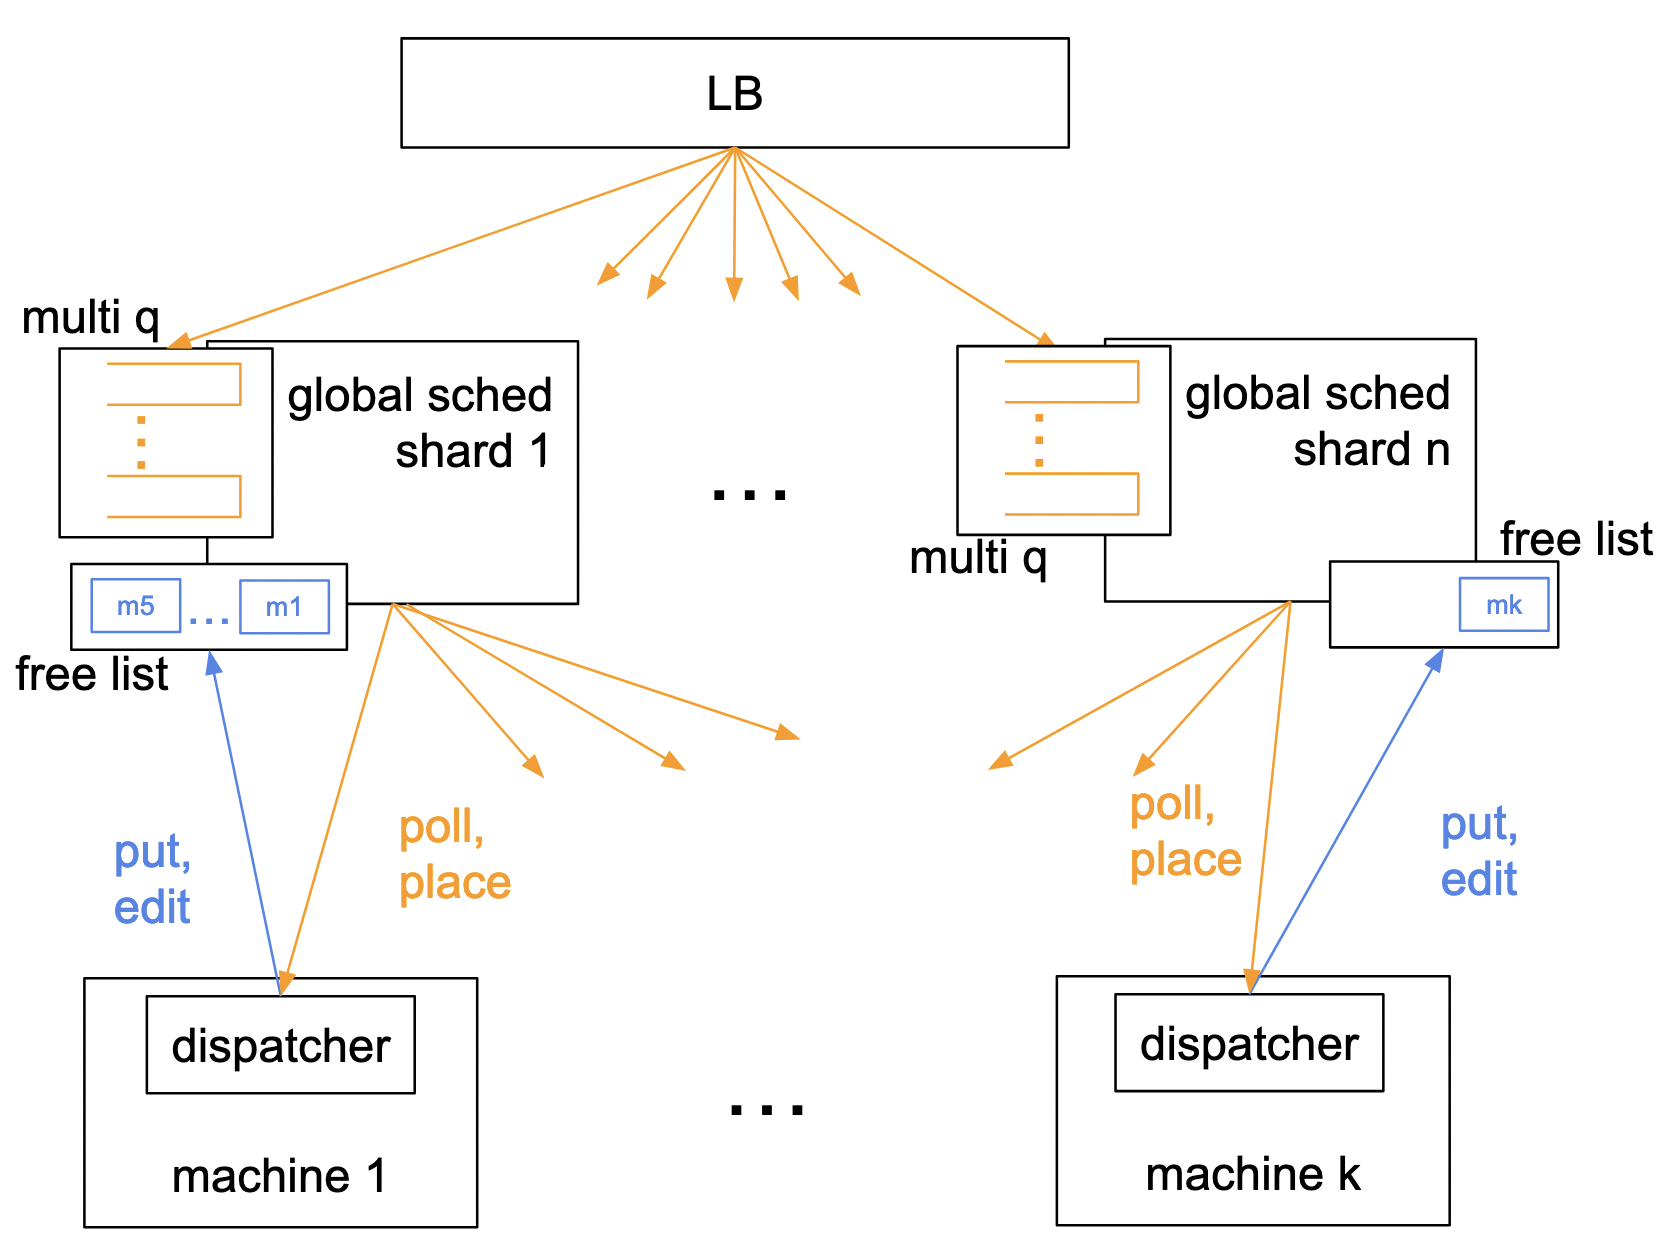
\includegraphics[width=9cm]{img/overview.png}
      \caption{ global scheduler shards queue and place jobs (in orange), 
      on each machine a dispatcher thread keeps track of memory utilization 
      and if it's low writes itself to an idle list (in blue) }
    \label{fig:overview}
\end{figure}
  

As shown in Figure~\ref{fig:overview}, \sys{} sits behind a load balancer, and
consists of: a distributed global scheduler, which places new function
invocations, a dispatcher, which runs on each machine and communicates with the
global scheduler shards, and a machine scheduler, which enforces priorities on
the machines.

Each global scheduler shard maintains an \textit{idle list}, which holds
machines that have a significant amount of memory available. In the shards idle
list each machine's entry is associated with the amount of free memory as well
as some information about compute pressure. This information allows the global
scheduler to place high priority processes quickly, without incurring the
latency overheads of finding available resources.

Global scheduler shards store the jobs waiting to be placed in a multi queue,
with one queue per priority.


\textbf{Machine Scheduler.}
The machine scheduler is a preemptive priority scheduler: it preempts lower
priority jobs to run higher priority ones. Being unfair and starving low
priority jobs is desirable in \sys{}, since image processing jobs should not
interrupt a page view request processing, but vice versa is expected.


\textbf{Dispatcher.}
The dispatcher is in charge of adding itself to a shard's idle list when memory
utilization is low. The dispatcher chooses which list to add itself to using
power-of-k-choices: it looks at k shards' idle lists and chooses the one with
the least other machines in it. If the machine is already on an idle list on
shard $i$, but the amount of available memory has changed significantly (either
by jobs finishing and memory being freed or by memory utilization increasing
because of new jobs or memory antagonists), the dispatcher will update shard
$i$'s idle list. These interactions from the dispatcher to free lists are
represented by the blue arrows in Figure~\ref{fig:overview}.

The dispatcher also responds to probes by shards: given a potential job that a
shard might want to run on the machine, the dispatcher computes the \textit{time
to profit}, which is the time it would take for the machine to start making a
profit off of the decision of placing the job there. If there is enough memory
free to fit the new job's max memory, that number is 0. If the dispatcher might
have to kill a process due to memory pressure, it computes which job it would
kill, which is the job with minimal price where $j.memUsg > newJ.maxMem$. The
time to profit then is $(jToKill.timeRun \cdot jToKill.price) / (newJ.price
- jToKill.price)$.

The dispatcher is also in charge of killing jobs under memory pressure, should
it occur. It chooses the job to kill by looking at both memory used and money
wasted if killed (lower priority jobs should be the ones to be killed if
possible, but won't help much if they weren't using any memory to begin with).
The dispatcher requeues killed jobs at a randomly chosen shard.

\makeatletter
\renewcommand{\ALG@name}{Procedure}
\makeatother
\begin{algorithm}[t]
\caption{Choosing a machine for a job j}\label{alg:place}
\begin{algorithmic}
    \State$N = \{ $ machines in freeList with memAvail > j.maxMem $\}$
    \If{$|N| > 0$} \\
        \Return$ $min(N.maxPriorityRunning, N.qSize)
    \EndIf
    \State$M = $ timeToProfit of k polled machines
    \If{min(M.timeToProfit$) < THRESH$} \\
        \Return$ $min($M$)
    \Else
        \State$ $reQ j, with priority -= 1
    \EndIf
\end{algorithmic}
\end{algorithm}


\textbf{Global Scheduler Shards.}

Shards choose what job to place next by looking at each job at the head of a
queue in the shards multi-queue, and comparing the ratio of priority to amount
of time spent in the queue. This ensures that high priority jobs don't have to
wait as long as lower priority jobs to be chosen next, but low priority jobs
will get placed if they have waited for a while.

When placing the chosen job, the shard finds a machine to run it, shown in
Procedure~\ref{alg:place}. The shard will first look in its idle list for a
machine that has the job's maximum memory available. If there are multiple such
machines, the shard looks at each machines compute pressure metrics; the goal
being to minimize cpu idleness and job latency in low load
settings.\hmng{playing with details of this in the scheduler right now} 

If a machine from the idle list is chosen, the response from the dispatcher upon
placing the job will include updated utilization information, which the shard
will use to update the idle list entry.

If there are no machines in the idle list with the memory available, the shard
switches over to power-of-k-choices: it polls k machines, sending the price and
the maximum memory of the job currently being placed, and getting back the time
to profit. The shard then can choose to place the new job on the machine with
the minimum value, or if all of them are too high the shard re-queues the job.
